\chapter{Local invariant features II}
\section{Difference of Gaussians (DoG)}
It is possible to define an approximation of the Laplacian of Gaussian by using difference of Gaussians:
\[DoG = G(x,y,k\sigma) - G(x,y,\sigma)\]
where $k$ is a scalar value and $G$ is the two-dimensional Gaussian function
\[\frac{1}{2\pi \sigma^{2}}e^{-\frac{x^{2} + y^{2}}{2\sigma^{2}}}\]
Basically, it approximates the behavior of the Laplacian of Gaussian computing the difference between two Gaussian functions with different values of $\sigma$
\begin{center}
    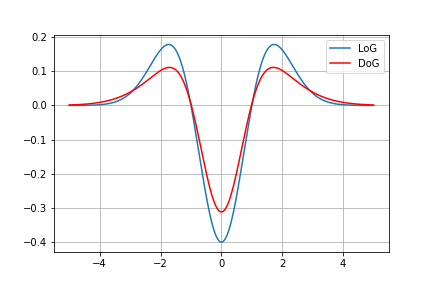
\includegraphics[scale = 0.7]{images/DoG Approx.png}
\end{center}
This is useful because $DoG$ is more efficient from a computational point of view. In fact, computing the second order derivative is more expensive than performing a difference between two functions.
\section{SIFT algorithm}
SIFT is a scale invariant feature detection algorithm that applies $DoG$ both in space and over different scales. Thanks to this, it is computationally more efficient than the Harris-Laplacian algorithm. Following are the major stages of computation used to generate the set of image features:
\begin{enumerate}
    \item \textbf{Scale-space extrema detection:} The first stage of computation searches for local features over all scales and image locations using a difference of Gaussian function.
    \item \textbf{Key-point localization:} At each candidate location, a detailed model is fit to determine location and scale. Key-points are selected based on measures of their stability (\textbf{It was not covered in class}).
    \item \textbf{Orientation assignment:} One or more orientations are assigned to each key-point location based on local image gradient directions.
    \item \textbf{Key-point descriptor:} Describing the key-points as a high dimensional vector such that it is highly distinctive and invariant as possible to variations such as changes in viewpoint, illumination, translation, rotation and scale.
\end{enumerate}
\begin{center}
    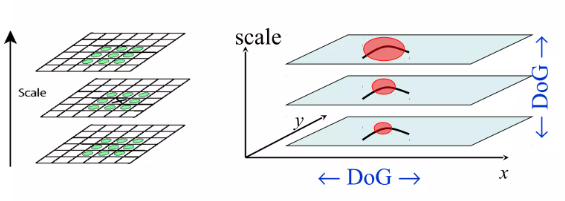
\includegraphics[]{images/DoG space scales.png}
\end{center}
\subsection{Scale-space peak Selection}
The initial image is repeatedly convolved with Gaussians with different values of $\sigma$ to produce a set of scale-space images. Adjacent Gaussian images are subtracted to produce the difference of Gaussian images. These $DoG$ images contain the details of the original image at different scales\footnote{look at the Sharpening filter and derivative of Gaussian sections}. This procedure creates the first \textbf{ octave of scale-space}. In order to find a good approximation of the Laplacian of Gaussian, this process is repeated multiple times and after each octave the Gaussian image is down-sampled by a factor of 2 (each octave’s image size is half the previous one).
\begin{center}
    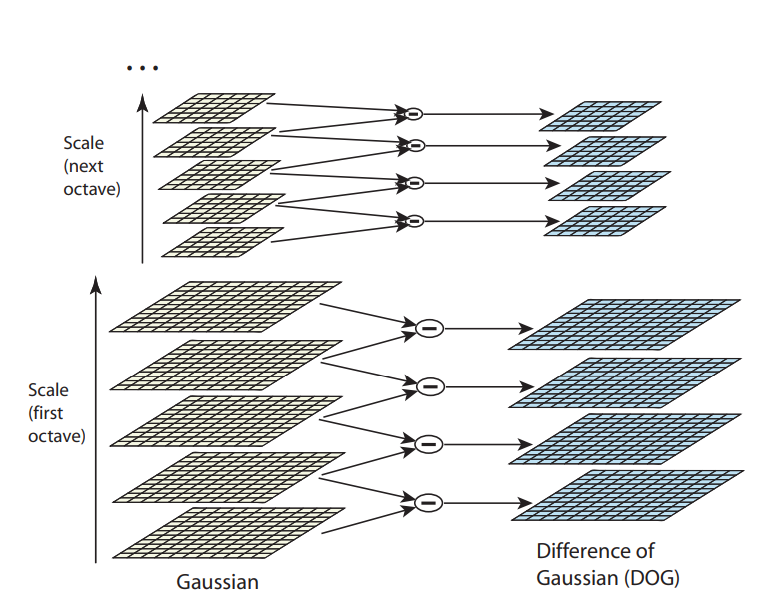
\includegraphics[scale = 0.9]{images/SIFT octaves.png}
\end{center}
Maxima and minima of the $DoG$ images are detected by comparing a pixel to its 26 neighbors in 3x3 regions at the current and adjacent scales (previous and next scales with respect to the current). A key-point is selected only if it is larger, in term of intensity, than all of these neighbors or smaller than all of them.
\begin{center}
    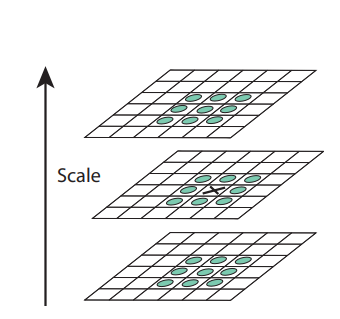
\includegraphics[]{images/SIFT DoG space.png}
\end{center}
Thanks to this, the local features detected are more robust also to some transformations across scales.
\subsection{Orientation assignment}
\label{subsection:orientation}
After the detection process we already know the scale at which each key-point was detected (parameter $\sigma$), so we have scale \textit{invariance}. By assigning a consistent orientation to each key-point based on local image properties, the
key-point descriptor can be represented relative to this orientation and therefore achieve invariance to image rotation.\newline\newline
An orientation histogram is formed from the gradient orientations of sample points within a region around the key-point (using the scale of the key-point to select the level of Gaussian blur for the image). The orientation histogram covers the 360 degree range of orientations. Each sample point added to the histogram is weighted by its gradient magnitude and by a Gaussian-weighted circular window. The highest peak in the histogram is selected as the dominant direction of the key-point and then any other local peak that is within 80\% of the highest peak is used to also create a key-point with that orientation. Therefore, for locations with multiple peaks of similar magnitude, there will be multiple key-points created at the same location and scale but different orientations.
\subsection{Key-point descriptor}
At this point, each key-point has a location, scale and orientation. The next step is to compute a descriptor for the local image region. To do this, a $16 \times 16$ window around the key-point is taken and it is divided into 16 sub-blocks of $4 \times 4$ size \footnote{The size of the window can be modified, $16 \times 16$ is the standard SIFT }. For each sub-block, an 8 bin orientation histogram is created following the procedure mentioned before (\ref{subsection:orientation}). Therefore, a descriptor will be a $4 \times 4 \times 8 = 128$ element feature vector.
\begin{center}
    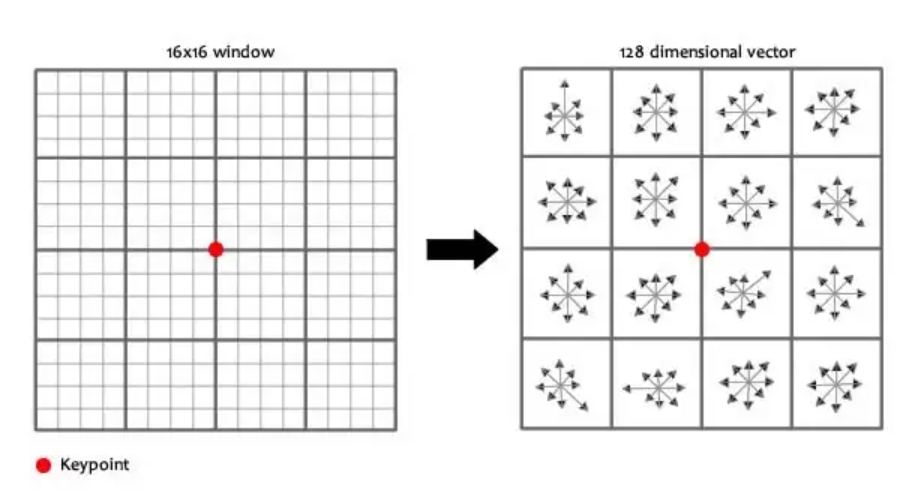
\includegraphics[scale = 0.7]{images/sift descriptor.png}
\end{center}
The feature vector uses gradient orientations, but if you rotate the image, these orientations change. So, in order to achieve orientation
invariance, the coordinates of the descriptor and the gradient orientations are rotated relative to the key-point orientation.
\subsection{Key-points matching}
A comparative evaluation of different scale invariant key-points detectors can be done by using the repeatability rate. It is defined as the ratio between the number of point-to-point correspondences that can be established for detected points and the number of all possible correspondences.
\begin{center}
    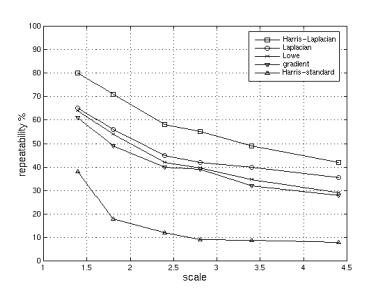
\includegraphics[scale = 1.3]{images/repeatability rate.png}
\end{center}
But how can we match key-points? One way to do it is by computing, for each descriptor in the first image, the Euclidean distance between this descriptor and all the descriptors of the second image and select the one with minimum distance. A more robust method can be, instead of looking only for the minimum distance, compute the ratio between the first two closest distances. If it is greater that 0.8, the match is rejected. 
\begin{center}
    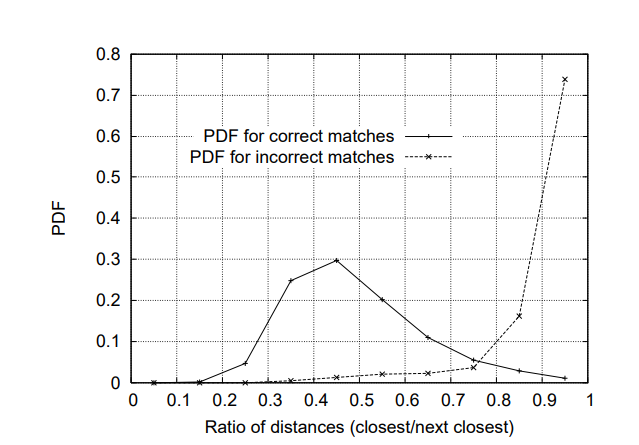
\includegraphics[]{images/ratio closest distances.png}
\end{center}
Now we can describe a pipeline to perform features matching:
\begin{enumerate}
    \item Detect key-points
    \item Build key-points descriptors
    \item Match key-point features
    \item Align images
\end{enumerate}

